\documentclass[xcolor=svgnames, colorlinks, handout]{beamer}
%\documentclass[xcolor=svgnames, handout]{beamer}

%\includeonlyframes{current}

\usepackage[utf8]    {inputenc}
\usepackage[T1]      {fontenc}
\usepackage[english] {babel}

\usepackage{amsmath,amsfonts,graphicx}
\usepackage{beamerleanprogress}
\usepackage{xcolor}
\usepackage{soul}
%\usepackage{verbatim}
\usepackage{multicol}
\usepackage{tikz} 
\usepackage[export]{adjustbox}
\usepackage{array}


\definecolor{iyellow}{RGB}{255, 162, 23}
\definecolor{sgreen}{RGB}{118, 191, 138}

\newcommand{\yellow}[1]{\textcolor{iyellow}{#1}}
\newcommand{\red}[1]{\textcolor{red}{#1}}
\newcommand{\green}[1]{\textcolor{ForestGreen}{#1}}
\newcommand{\blue}[1]{{\textcolor{blue}{#1}}}
\newcommand{\purple}[1]{{\textcolor{purple}{#1}}}
\newcommand{\orange}[1]{{\textcolor{orange}{#1}}}
\newcommand{\bblue}[1]{\textcolor{SteelBlue!90!gray}{#1}} % beamer blue
\newcommand{\tans}[2]{\textbf<#1>{\textit<#1>{{\color<#1>{iyellow}{#2}}}}}

\newcommand{\eol}{\\[1em]\pause}
\newcommand{\nl}{\\[1em]}
\newcommand{\define}[1]{\textbf{\textcolor{orange}{#1}}}
\newcommand{\answer}[1]{\textit{\textbf{\textcolor{iyellow}{#1}}}}
\newcommand{\command}[1]{\texttt{\textbf{\textcolor{DarkMagenta}{#1}}}}
\newcommand{\ipic}[2]{\includegraphics[width={#2}\textwidth]{#1}}
\newcommand{\cell}[1]{{\sf \textbf{\textcolor{DarkMagenta}{#1}}}}
\newcommand{\ra}{$\rightarrow$}
\newenvironment{allintypewriter}{\ttfamily}{\par}


\hypersetup{
    colorlinks=true,
    linkcolor=blue,
    filecolor=magenta,      
    urlcolor=cyan,
}
 

            

\setbeamertemplate{theorems}[numbered] 
 \setbeamersize{description width=0.57cm} % to have less indent with the description environment


\newcommand{\ft}[1]{\frametitle{#1}}
\usepackage{fancyvrb}

\usepackage{upquote,textcomp}

\newcommand{\bs}{$\backslash$}

\usepackage[T1]{fontenc}
\usepackage[utf8]{inputenc}
\usepackage{tikz}
\usetikzlibrary{shadows}

\newcommand*\keystroke[1]{%
  \tikz[baseline=(key.base)]
    \node[%
      draw,
      fill=white,
      drop shadow={shadow xshift=0.25ex,shadow yshift=-0.25ex,fill=black,opacity=0.75},
      rectangle,
      rounded corners=2pt,
      inner sep=1pt,
      line width=0.5pt,
      font=\scriptsize\sffamily
    ](key) {#1\strut}
  ;
}

\title
  [Data 301 Data Analytics\hspace{2em}]
  {Data 301 Data Analytics\\
An Introduction to Python}

\author
  [Dr.\ Irene Vrbik]
  {Dr.\ Irene Vrbik}

\date
  {Term 1, 2018}

\institute
  {University of British Columbia Okanagan \newline irene.vrbik@ubc.ca}


\graphicspath{{img/}}

\begin{document}

\maketitle

\setbeamersize{description width=0.57cm} % to have less indent with the description environment

\begin{frame}\ft{Why learn Python?}
Python is increasingly the most popular choice of programming language for data analysts because it is designed to be simple, efficient, and easy to read and write.\nl

There are many open source software and libraries that use Python and data analysis tools built on them. \nl

We will use Python to learn programming and explore fundamental programming concepts of commands, variables, decisions, repetition, and events.

\end{frame}


\begin{frame}\ft{What is Python?}
Python is a general, high-level programming language designed for code readability and simplicity.\nl

Python is available for free as open source and has a large community supporting its development and associated tools.\nl

Python was developed by Guido van Rossum and first released in 1991.  Python 2.0 was released in 2000 (latest version 2.7), and a backwards-incompatible release Python 3 was in 2008.
\begin{itemize}
\item Our coding style will be Python 3 but most code will also work for Python 2.
\item (P.S. the name comes from Monty Python)
\end{itemize}
\end{frame}


%features: https://www.javatpoint.com/python-features
\begin{frame}\ft{Python Language Characteristics}
Python supports:
\begin{itemize}
\item \href{https://pythonconquerstheuniverse.wordpress.com/2009/10/03/static-vs-dynamic-typing-of-programming-languages/}{dynamic typing}  -- types can change at run-time
\item \href{https://blog.newrelic.com/engineering/python-programming-styles/}{multi-paradigm}  -- flexible in that is supports both procedural, object-oriented, and functional styles, for example.
\item automatic \href{https://www.youtube.com/watch?v=URNdRl97q_0}{memory management} and  \href{https://rushter.com/blog/python-garbage-collector/}{garbage collection}
%\item extendable -- small core language that is easily extendable
\item extensible --  other languages such as C/C++ can be used to compile the code.
\item and \href{https://data-flair.training/blogs/features-of-python/}{more ...}
\end{itemize}
\end{frame}

\begin{frame}\ft{Python Language Characteristics}
Python core philosophies (by \href{https://www.python.org/dev/peps/pep-0020/}{Tim Peters})
\begin{itemize}
\item Beautiful is better than ugly
\item Explicit is better than implicit
\item Simple is better than complex
\item Complex is better than complicated
\item Readability counts
\end{itemize}
\end{frame}


%\begin{frame}[fragile]\ft{Some Quotes}
%it
%%If you can't write it down in English, you can't code it.
%
%%������������������� -- Peter Halpern
%%\begin{quote}
%%If you lie to the computer, it will get you.
%%\end{quote}
%%������������������� -- Peter Farrar�
%%
%\end{frame}

\begin{frame}\ft{Some Quotes}
\begin{quote}
If you can't write it down in English, you can't code it.
\end{quote}
\hfill --- Peter Halpern

%\begin{quote}
%If you lie to the computer, it will get you.
%\end{quote}
%\hfill --- Peter Farrar

\begin{quote}
I really hate this damn machine.\\
I wish that I could sell it.\\
I never does quite what I want.\\
Just only what I tell it.
\end{quote}
\hfill --- programmers lament

\end{frame}

\begin{frame}\ft{Introduction to Programming}
{\it Recall\dots}\nl
An \emph{algorithm} is a precise sequence of steps to produce a result.  A \emph{program} is an encoding of an algorithm in a \define{language} to solve a particular problem.\nl

There are numerous languages that programmers can use to specify instructions.  Each language has its different features, benefits, and usefulness.\nl

The goal is to understand fundamental programming concepts that apply to all languages.

\end{frame}


\begin{frame}{Installing and Using Python}

Follow \href{https://wiki.python.org/moin/BeginnersGuide/Download}{this} guide on getting Python 3 on your computer (or \href{https://realpython.com/installing-python/}{this} guide, or \href{https://wsvincent.com/install-python3-mac/}{this} guide (for Macs),  or countless others you might find on the internet). \\

\bigskip

Another way you can get python is through \href{https://www.anaconda.com/distribution/}{Anaconda} (recommended).
\begin{itemize}
\item See \href{https://www.youtube.com/watch?v=LrMOrMb8-3s}{this} help video (Windows)
\item See \href{https://www.youtube.com/watch?v=YJC6ldI3hWk}{this} help video (Mac)
\end{itemize}

\end{frame}



\begin{frame}[fragile]\ft{Python: Basic Rules}
\begin{itemize}
\item To program in Python you must follow a set of rules for specifying your commands.  This set of rules is called a \define{syntax}.
\begin{itemize}
\item Just like any other language, there are rules that you must follow if you are to communicate correctly and precisely.\nl
\end{itemize}
\item For a more thorough overview of Python, you may have a look at \href{https://www.bogotobogo.com/python/files/pytut/Python%20Essential%20Reference,%20Fourth%20Edition%20(2009).pdf}{Python Essential Reference by David Beazley} as well as countless website online, eg \href{https://www.w3schools.com/python/}{w3schools}, \href{https://www.codecademy.com/learn/learn-python-3}{codeacademy}, \dots
\medskip

\item Other useful resources include: \href{https://docs.python.org/3/}{documentation for Python 3.7.3}, 
\href{https://www.python.org/about/gettingstarted/}{Python.org (getting started)}, \href{https://www.w3schools.com/python/}{w3schools} \href{https://www.w3schools.in/python-tutorial/}{and tutorials} 
 and the \href{https://www.python.org/dev/peps/pep-0008/}{Pep 8 style guide}.
\end{itemize}
\end{frame}


\begin{frame}[fragile]\ft{Python: Basic Rules}

Important general rules of Python syntax:
\begin{itemize}
\item Python \emph{is} case-sensitive.
\item Python \emph{is} particular on whitespace and indentation.
\item The end of command is the end of line (i.e semi-colons are not a required terminator).
\item Use four spaces for indentation whenever in a block.
\begin{itemize}
%https://www.python.org/dev/peps/pep-0008/#indentation
\item Spaces are the preferred indentation method.
\item Tabs should be used solely to remain consistent with code that is already indented with tabs.
\item Python 3 disallows mixing tabs and spaces for indentation.
\end{itemize}

\end{itemize}
\begin{verbatim}
    def spam():
        eggs = 12
        return eggs
    print spam()
\end{verbatim}



\end{frame}

\begin{frame}[fragile]\ft{Comments}
\define{Comments} are used by the programmer to document and explain the code.  Comments are ignored by the computer. \nl %Two types:
%\begin{enumerate}
%\item {\bf One line comment}: put ``\command{\#}" before the comment and any characters to the end of line are ignored by the computer.
%%\item {\bf Multiple line comment}: put \command{"""} at the start of the comment and \command{"""} at the end of the comment.  The computer ignores everything between the start and end comment indicators.
%\end{enumerate}
Type \command{\#} before the comment and any characters to the end of line are ignored by the computer.
Example:
\begin{Verbatim}[frame=single]
# Single line comment
print (1)  # Comment at end of line
\end{Verbatim}
%""" This is a 
%multiple line
%comment """
\end{frame}

\begin{frame}[fragile]\ft{Python Programming}
A Python program, like a book, is read left to right and top to bottom.
Each command is on its own line.
\begin{Verbatim}[frame=single]
# Sample Python program
name = "Joe"
print("Hello")
print("Name: "+name)
\end{Verbatim}

A user types in a Python program in a text editor (\href{https://wiki.python.org/moin/PythonEditors}{some examples}%. \href{https://www.sublimetext.com/}{Sublime Text}
) or integrated development environment (\href{https://wiki.python.org/moin/IntegratedDevelopmentEnvironments}{IDE examples}).\\
%and then runs the program.
\medskip
To run the  program we need a Python \emph{interpreter} (i.e. a program that reads Python programs and carries out their instructions).

\end{frame}


\begin{frame}{Installing and Using Python}
% https://opentechschool.github.io/python-beginners/en/getting_started.html
You may already have a version of python on your computer.  \nl
You can check by opening the command window/terminal and typing {\tt py}/{\tt python} (Windows/Mac).\nl
To exit using Python in the console type \keystroke{Ctrl} + keystroke{Z}  then \keystroke{ENTER} (if using Windows) or \keystroke{Ctrl} + keystroke{D} on a Mac.\nl
Alternatively, you could also run the python command {\tt exit()}.\nl
Read more about running python through the console \href{https://opentechschool.github.io/python-beginners/en/getting\_started.html}{here}.\nl
You could also use one of the various \href{https://www.tutorialspoint.com/execute_python3_online.php}{online Python 3 compilers} for example.
\end{frame}


\begin{frame}{Installing and Using Python}
\begin{alertblock}{Python version}
If you haven't done any of the installations above, this is probably going to be Python 2.
\end{alertblock}
\ipic{img/pythonshell.png}{0.99}\\
You can find out which version of Python you have by typing {\tt python -V} %or {\tt python --version}
 in your console.
\end{frame}



\begin{frame}\ft{Python Editor - Jupyter}
``\href{https://jupyter.org/}{Project Jupyter} exists to develop open-source software, open-standards, and services for interactive computing across dozens of programming languages.''\nl
\define{Jupyter} notebook is a graphical, browser-based application for editing and running  Python.
% allows us to code in a web browser
Follow the instructions \href{http://jupyter.org/install}{here} to install.\nl
To run, type {\tt jupyter notebook} in your Command Prompt.\nl
This action will start the notebook server in your default browser and echo information about the notebook server in your terminal.\nl
Read more about it by clicking {\it Try Jupyter for Python} \href{https://jupyter.org/try}{here}
\end{frame}




\begin{frame}\ft{Python Editor - Jupyter}
The \emph{Notebook Dashboard} will list all of the notebooks (.ipynb), files, and subdirectories stored in the \emph{local} working directory (i.e. the directory from which you launched jupyter)
$$\ipic{img/jnote}{0.8}$$
\end{frame}





\begin{frame}\ft{Python Editor - Jupyter}

To create anew notebook, select {\bf New,  Python3}.
\begin{center}
\ipic{img/jupyter}{0.8}
\end{center}
\end{frame}

\begin{frame}\ft{Python Editor - Jupyter}
To close this program, navigate the the {\bf Running} tab and click the orange Shutdown button {\bf  Closing the notebook's page is not sufficient to shutdown}.
\begin{center}
\ipic{img/shutdown}{0.8}
\end{center}
\end{frame}


\begin{frame}\ft{Python Editor -- jupyter notebook}
\begin{center}
\ipic{img/jupyterbutton}{0.98}
\end{center}

\end{frame}


\begin{frame}\ft{Python Editor -- jupyter notebook}
\begin{itemize}
\item The body of the notbook is comprised of \emph{cells}:
\begin{description}
\item[Markdown cells] are used to build write regular (non-code) text. More markdown \href{https://github.com/adam-p/markdown-here/wiki/Markdown-Cheatsheet}{here} and see helpful \href{https://guides.github.com/pdfs/markdown-cheatsheet-online.pdf}{cheatsheet}.
\item[Code cells (default)]  are used to define the code which will be compiled (after pressing 
\includegraphics[height=1em]{img/run} or pressing \keystroke{Shift} + \keystroke{Enter}) to produce output.\nl
\end{description}

\item You can inserts cells (either code/markdown) anywhere by clicking {\bf Insert} $>$ {\bf Insert Cell Above} (or {\bf Insert Cell Below})
\medskip
\item Same thing goes for deleting/copying/pasting/undoing cells: see the  {\bf Edit} drop down menu bar.
\end{itemize}


\end{frame}



\begin{frame}\ft{Python Editor -- jupyter notebook}
You can create regular text and headings in markdown mode.  Headings are indicated using {\tt \#} (subheadings use {\tt \#\#})
\begin{center}
\ipic{img/textbefore}{0.98}
\end{center}
\end{frame}

\begin{frame}\ft{Python Editor -- jupyter notebook}
This is what the markdown looks like after it is run:
\begin{center}
\ipic{img/textafter}{0.98}
\end{center}
\end{frame}


\begin{frame}\ft{Python Editor -- jupyter notebook}
After a cell is run, a number will appear in the square parenthesis (an asterisk {\tt *} will appear for cells that are currently running).  Every time we run that cell, this number will increase.
\begin{center}
\ipic{img/runnum}{0.98}
\end{center}
\end{frame}

\begin{frame}\ft{Python Editor -- jupyter notebook}
\begin{itemize}
\item While jupyter notebook does autosave periodically, it is a good to save your work upon exiting (go to {\bf File} $>$ {\bf Save and Checkpoint} or click the save icon).\nl
\item  When we open the file again, it is not guaranteed that everything we need is in memory.\nl
\item It is good practice to ``reset" the session by clicking {\bf Kernel} $>$ {\bf Restart and Run all Cells} to ensure everything we need has been loaded into our working session (note that this will reset all of our numbers in the square brackets).
\end{itemize}
\end{frame}


\begin{frame}[fragile]\ft{Python: Hello World!}
A \href{https://en.wikipedia.org/wiki/\%22Hello,_World!\%22_program}{traditional introduction} into programming involves outputting the message {\verb|"Hello World!"|}\nl

In Python3, this is a simple as typing:
\begin{Verbatim}[frame=single]
print("Hello World!")
\end{Verbatim}
\vspace{1em}
The {\tt print} function will print to the terminal (standard output) whatever data (number, string, variable) it is given.\nl
You can use double quotes (\verb|"Hello world"|) or single quotes (\verb|'Hello world'|) just be consistent! E.g. \verb|'Hello World!"| will produce a error.
\end{frame}

\begin{frame}[fragile]\ft{Tripple Quotes}
\begin{itemize}
\item If your message runs across multiple lines, you can use 3 quotations to denote multi-line strings.\nl
\item The sting begins with a \verb|'''| (or \verb|"""|) and ends with a (or \verb|"""|).\nl
\item Note that in this environment, we can use linebreaks (ie we can start a new line by pressing ENTER) and include the single and double quotes with our string.
\end{itemize}
$$\ipic{img/tripplequotes}{0.6}$$
\end{frame}



\begin{frame}[fragile]\ft{Try It: Python Printing}
\begin{example}
 Write a Python program that prints "I can start coding!"
 \end{example}

\begin{example}
 Write a Python program that prints these three lines:
 \begin{verbatim}
I know that I can program in Python.
I am programming right now.
My awesome program has three lines!
 \end{verbatim}
\end{example}


\end{frame}

%%%%%%%%%%%%%%%%%%%%%%%%%

% question:

\begin{frame}[fragile]\ft{}
  \begin{example}
How many of the following statements are TRUE?
\begin{enumerate}
\item {{Python is case-sensitive.}}
\item {{A command in Python must be terminated by a semi-colon.}}
\item {{Indentation does not matter in Python.}}
\item {{A single line comment starts with \verb|"""|.}} 
\item {{The print command prints to standard input.}}
\end{enumerate}
\begin{multicols}{5}
\begin{enumerate}[A)]
\item 0 
\item 1
\item 2
\item 3
\item 4
\end{enumerate}
\end{multicols}
  \end{example} 
\end{frame}


% answer:

\begin{frame}[fragile]\ft{}
  \begin{block}{Answer:}
How many of the following statements are TRUE?
\begin{enumerate}
\item {\color<1->{sgreen} {Python is case-sensitive.}}
\item {\color<2->{red}{A command in Python must be terminated by a semi-colon.}}
\item {\color<3->{red}{Indentation does not matter in Python.}}
\item {\color<4->{red}{A single line comment starts with "\verb|"""|".}} 
\item {\color<5->{red}{The print command prints to standard input.}}
\end{enumerate}
\begin{multicols}{5}
\begin{enumerate}[A)]
\item 0 
\item \tans{5}{1}
\item 2
\item 3
\item 4
\end{enumerate}
\end{multicols}
  \end{block} 
\end{frame}



%%%%%%%%%%%%%%%%%%%%%%%%%



\begin{frame}[fragile]\ft{Variables}
\textit{Recall\dots}\nl
A \emph{variable} is a name that refers to a location that stores a data value.
$$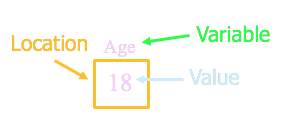
\includegraphics[]{../04VBA/img/Variable.png}$$
\begin{alert}
{IMPORTANT:} The \emph{value} at a location can change using initialization or assignment.
\end{alert}
\end{frame}



\begin{frame}[fragile]\ft{Variable Assignment}
\begin{columns}[T] % align columns
\begin{column}{.48\textwidth}
In python the \define{assignment} operator is ``\command{=}".\nl
We will use it to (re)set value of a variable.
\begin{itemize}
\item Example:
\begin{verbatim}
num = 10
message = "Hello world!"
\end{verbatim}
\end{itemize}
\end{column}%
\hfill%
\begin{column}{.3\textwidth}
\ipic{variables}{1.3}
\end{column}%
\end{columns}
\end{frame}

\begin{frame}[fragile]\ft{Python Variables}
%To create a variable in Python, you must only provide a name.\nl
Variables are created when first assigned.\nl
%Unlike other programming languages, Python has no command for declaring a variable.

A variable type is dynamic and do not need to be declared.\nl
  It can store any particular type (e.g.  int, float, strings, or Boolean) at any given time.
  \begin{itemize}
\item Example:
\begin{verbatim}
val = 5
val = "Hello"
isAwesome = True
\end{verbatim}
  \end{itemize}
Recall: \define{Boolean} values can be either True or False.  N.B. in Python \alert{case matters}.\nl
%\begin{verbatim}
%isAwesome = False
%\end{verbatim}
The type (string, int, float etc.) of the variable is determined by Python.
\end{frame}
% https://www.w3resource.com/python/python-variable.php

\begin{frame}\ft{Variable Rules}
Variables are a name that must begin with a letter or an underscore and cannot contain spaces.  All subsequent characters must be letters, numbers or underscores. \nl
Variables are created when they are first used. There is no special syntax to declare (create) a variable.\nl
Variable names \alert{are} case-sensitive.   \nl
A programmer picks the names for variables, but try to make the names meaningful and explain their purpose.\nl
Avoid naming variables as reserved words (e.g. {\tt if, for, else}).  A reserved word has special meaning in the language.
\end{frame}


% question:

\begin{frame}\ft{}
  \begin{example}
How many of the following variable names are valid?
\begin{enumerate}
\item {	{name}}
\item {	{string2}}
\item {	{2cool}}
\item {	{under\_score}} 
\item {	{space name}} 
\item {	{else}} 
%\item {{\_test}} 
\end{enumerate}
\begin{multicols}{5}
\begin{enumerate}[A)]
\item 0 
\item 1
\item 2
\item 3
\item $\geq$ 4
\end{enumerate}
\end{multicols}
  \end{example} 
\end{frame}


% answer:

\begin{frame}<handout:0>\ft{}
  \begin{block}{Answer:}
How many of the following variable names are valid?
\begin{enumerate}
\item {\color<1->{sgreen}	{name}}
\item {\color<2->{sgreen}	{string2}}
\item {\color<3->{red}	{2cool}}
\item {\color<4->{sgreen}	{under\_score}} 
\item {\color<5->{red}	{space name}} 
\item {\color<6->{red}	{else}} 
%\item {\color<7->{green}	{\_test}} 
\end{enumerate}
\begin{multicols}{5}
\begin{enumerate}[A)]
\item 0 
\item 1
\item 2
\item \tans{6}{3}
\item $\geq$ 4
\end{enumerate}
\end{multicols}
  \end{block} 
\end{frame}




\begin{frame}[fragile]\ft{Python Math Expressions}
Math expressions in Python: 
\begin{center}
\begin{tabular}{|c|c|c|c|}\hline
\textbf{Operation} & {\bf Syntax} & {\bf Example} & {\bf Output}\\\hline
Add
& +
& 5 + 3 & 8 \\
Subtract
& -
& 10 - 2 & 8 \\
Multiply
& *
& 5 * 3 & 15\\
Divide
& /
& 8/4 & 2  \\
Modulus
& \% 
& 9 \% 4
& 1 \\
Exponent &
**&
5 ** 2 &
 25\\\hline
\end{tabular}
\end{center}
\end{frame}

\begin{frame}\ft{Expressions - Operator Precedence}
Each operator has its own priority similar to their priority in regular math expressions:
\begin{enumerate}
\item Any expression in parentheses is evaluated first starting with the inner most nesting of parentheses.
\item Exponents
\item Multiplication and division (*, /, \%) 
\item Addition and subtraction (+,-)\nl
\end{enumerate}

Recall: \define{BEDMAS} \emph Brackets \emph Exponents \emph Division, \emph Multiplication, (modulus), \emph Addition and \emph Subtraction

\green{Example:} {\tt 20 - \orange(\blue(4 + 5\blue) - \blue(3 * \red(6 - 2\red)\blue)\orange) * 4} = 32

\end{frame}

\begin{frame}\ft{Python Expression Question}
\begin{example}
What is the value of this expression 
$${\tt 8 ** 2 + 12 / 4 * (3 -1) \% 5}$$
HINT: Modulo is executed after multiplication and division; more on this \href{https://en.wikipedia.org/wiki/Order_of_operations\#Programming\_languages}{here}.
\end{example}
\begin{multicols}{5}
\begin{enumerate}[A)]
\item 69
\item 65
\item 36
\item 16
\item 70
\end{enumerate}
\end{multicols}
\end{frame}


\begin{frame}<handout:0>[fragile]\ft{Python Expression Question}
\begin{block}{Answer:}
What is the value of this expression 
$${\tt 8 ** 2 + 12 / 4 * (3 -1) \% 5}$$
HINT: Modulo is executed after multiplication and division; more on this \href{https://en.wikipedia.org/wiki/Order_of_operations\#Programming\_languages}{here}.
\end{block}
\begin{multicols}{5}
\begin{enumerate}[A)]
\item 69
\item \tans{1}{65}
\item 36
\item 16
\item 70
\end{enumerate}
\end{multicols}
I think it's good practice to be explicit with brackets. I.e., I might have written the above as:
\begin{center}
\begin{minipage}{6cm}
\begin{Verbatim}[frame=single]
8**2 + ((12/4)*(3-1))%5
\end{Verbatim}
\end{minipage}
\end{center}
\end{frame}



\begin{frame}\ft{Try it: Python Variables and Expressions}
\begin{example}
Write a program that prints the result of {\tt 35 + 5*10}
\end{example}
\begin{example}
Write a program that uses at least 3 operators to end up with the value 99.
\end{example}
\begin{example}
Write a program that has a variable called name with the value of your {\tt name} and a variable called {\tt height} storing your height in feet.  Print out your name and {\tt height} using these variables.
\end{example}
\end{frame}

\begin{frame}[fragile]\ft{Rules for Stings in Python}
Strings are sequences of characters that must be surrounded by single or double quotes.\nl
Any number of characters is allowed.
The minimum number of characters is zero {\tt ""}, which is called the \define{empty string}.
\nl
Strings can contain most characters except enter, backspace, tab, and backslash. These special characters must be \emph{escaped} by using the escape character:  $\backslash$
\begin{itemize}
\item Example:
\begin{description}
\item [new line] {\tt $\backslash$n}
\item [single quote] $\backslash$\verb|'| 
\item [backslash] {\tt $\backslash$$\backslash$} 
\item [double quote] $\backslash$\verb|''| 
\end{description}
\end{itemize}
\end{frame}


\begin{frame}[fragile]\ft{Strings}
%Strings are sequences of characters that are surrounded by either single or double quotes.\nl
%Use the escape character ($\backslash$) for apostrophes e.g., \verb|There\'s|\nl
As mentioned previously, we can use triple  quotes \verb|"""| for a strings that contain single/double quotes and/or line breaks.\nl

In addition, double quoted strings can contain single quoted strings and vice versa. Example:\nl

%The use of the word "escape" really means to temporarily escape out of parsing the text and into a another mode where the subsequent character is treated differently.

\begin{verbatim}
name = ''Joseph "Joe" Jones'
storeName = 'Joe\'s Store'
storeName = "Joe's Store" # alternatively
height = '''5'9"'''
print("""String that is really long
with multiple lines
     and spaces is perfectly fine""")
\end{verbatim}
% String \emph{literals} (values) have the quotation marks removed when displayed.
\end{frame}

%\begin{frame}[fragile]\ft{Raw Stings in Python}
%A string in raw mode ({\tt r} before quote) a character following a backslash is included in the string without change, and all backslashes are left in the string
%%  May be useful if data contains escapes. 
%\begin{itemize}
%\item  Example:
%\begin{verbatim}
%>>> st = r"slash\n hello"
%>>> st2 = "slash\n hello"
%>>> print(st)
%slash\n hello
%>>> print(st2)
%slash
% hello
%\end{verbatim}
%\end{itemize}
%N.B. \verb|>>>| indicates input (lack of \verb|>>>| indicates output).
%\end{frame}
%
%\begin{frame}[fragile]\ft{Raw Stings in Python}
%Raw strings are \alert{\it not} the same as verbatim. A raw string cannot end in an odd number of backslashes since it will be treated as an escape character.  More on this \href{https://www.journaldev.com/23598/python-raw-string}{here}.\nl
%
%\begin{itemize}
%\item For example:
%\begin{verbatim}
%>>> print(r"\"")
%\"
%>>> print(r"\\")
%\\
%>>> print(r"\")
%  File "<stdin>", line 1
%    print(r"\")
%              ^
%SyntaxError: EOL while scanning string literal
%\end{verbatim}
%\end{itemize}
%\end{frame}



\begin{frame}[fragile]\ft{Python String Indexing}\label{str}
Individual characters of a string can be accessed using square brackets ({\tt []}); the first character indexed at 0.\nl
\begin{itemize}
\item Example:
\begin{verbatim}
str = "Hello"
print(str[1]) 			# e
print("ABCD"[0])		# A
print(str[-1])			# o 
# Negative values start at end and go backward
\end{verbatim}
\end{itemize}
Read all more about strings \href{https://www.python.org/dev/peps/pep-0498/}{here}.
\end{frame}


%%%%%%%%%%%%%%%%%%%%%%%%%

% question:

\begin{frame}[fragile]\ft{}
  \begin{example}
How many of the following are valid Python strings?
\begin{enumerate}
\item {\verb|""|}
\item {\verb|''|}
\item {\verb|"a"|}
\item {\verb|" "|}
\item {\verb|"""|}
\item {\verb|"Joe\' Smith\""|}
\end{enumerate}
\begin{multicols}{5}
\begin{enumerate}[A)]
\item 1
\item 2
\item 4
\item 5
\item 6
\end{enumerate}
\end{multicols}
  \end{example} 
\end{frame}


% answer:

\begin{frame}<handout:0>[fragile]\ft{}
  \begin{block}{Answer:}
How many of the following are valid Python strings?
\begin{enumerate}
\item {\color<1->{sgreen}	{\verb|""|}}
\item {\color<2->{sgreen}	{\verb|''|}}
\item {\color<3->{sgreen}	{\verb|"a"|}}
\item {\color<4->{sgreen}	{\verb|" "|}} 
\item {\color<5->{red}	{\verb|"""|}} 
\item {\color<6->{sgreen}	{\verb|"Joe\' Smith\""|}} 
\end{enumerate}
\begin{multicols}{5}
\begin{enumerate}[A)]
\item 1
\item 2
\item 4
\item \tans{6}{5} 
\item 6
\end{enumerate}
\end{multicols}
  \end{block} 
\end{frame}


%%%%%%%%%%%%%%%%%%%%%%%%%




\begin{frame}[t, fragile]\ft{Python String Functions and Methods}
Suppose: \begin{verbatim}
           st = "Hello"
           st2 = "Goodbye"
\end{verbatim}

\begin{center}
\begin{tabular}{|l| >{\ttfamily}c | >{\ttfamily}l  | >{\ttfamily}l |}\hline
\textbf{Operation} & {\bf Syntax} & {\bf Example} & {\bf Output}\\\hline
Length &
len() &
len(st) &
5\\\hline
Upper case &
upper() &
st.upper() &
HELLO\\\hline
Lower case &
lower() &
st.lower() &
hello\\\hline
Convert to a string &
str() &
str(9) &
"9"\\\hline
Concatenation &
+ &
st1 + st2 &
HelloGoodbye\\\hline
Substring &
[] &
st[0:3] &
Hel\\
 &
&
st[1:] &
ello\\\hline
String to int &
int() &
int("99") &
99\\\hline

\end{tabular}
\end{center}
\end{frame}


\begin{frame}{Dot Notation}
\begin{itemize}
\item Like VBA, you will notice that python uses the dot operator  to perform \emph{methods} on \emph{objects} (read more \href{https://python4astronomers.github.io/python/objects.html}{here}). \nl
\item Every constant, variable, or function in Python is actually a object with a type and associated attributes and methods. \nl
%\item An attribute a property of the object that you get or set by giving the <object_name> + dot + <attribute_name>, for example img.shape.
\item  A \define{method}  is a function that is attached to an object (read more about this \href{https://data-flair.training/blogs/python-method-and-function/}{here})\nl
%\item When calling a  method on an object,  it possibly makes changes to that object.\nl % when does it do this?
\item \href{https://www.w3schools.com/python/python\_ref\_string.asp}{Here} are some more examples of string methods.
\end{itemize}
\end{frame}



\begin{frame}[fragile]\ft{String Operators: Concatenation}
The \emph{concatenation operator} is used to combine two strings into a single string.  The notation is a plus sign ``\define{+}".

\begin{itemize}
\item 
Example:
\begin{Verbatim}[frame=single]
>>> st1 = "Hello"
>>> st2 = "World!"
>>> st3 = st1 + st2 # HelloWorld!
>>> print(st1+st1)
HelloHello
>>> print(st3)
HelloWorld!
\end{Verbatim}
\end{itemize}
\end{frame}


\begin{frame}[fragile]\ft{String Operators: Concatenation}
Note that we must hard code spaces if we want them:
\begin{Verbatim}[frame=single]
>>> st4 = st1 +" "+ st2 
>>> print(st4)
Hello World!
\end{Verbatim}
\begin{alertblock}{Concatenate with numbers and strings}
We must convert numbers to strings before concatenation.
\end{alertblock}

\begin{Verbatim}[frame=single]
>>> num = 5
>>> print(st1+str(num))         
Hello5
\end{Verbatim}
N.B. we can mix types in the {\tt print()} function, i.e. without concatenation. Notice how {\tt print()} inserts spaces between inputs:
\begin{Verbatim}[frame=single]
>>> print(st1,num, 100, "hi there", "byethere")  
Hello 5 100 hi there byethere
\end{Verbatim}
\end{frame}



\begin{frame}[fragile]\ft{String Operators: Deleting objects}
If you have been following along with me, you will find that the code on the previous slide does not work.\nl
This is because {\tt str} is no longer treated as a function because I assigned \verb|"Hello"| to this object on slide \ref{str}. \nl
To delete this object we can type:
\begin{Verbatim}[frame=single]
del str
\end{Verbatim}
Now we are free to use the \textit{function} {\tt str()} as desired.
\end{frame}


%%%%%%%%%%%%%%%%%%%%%%%%%

% question:

\begin{frame}[fragile]\ft{}
  \begin{example}
What is the output of this code?
\begin{verbatim}
st1 = "Hello"
st2 = "World!"
num = 5
print(st1 + str(num) + "  " + st2)
\end{verbatim}
\begin{enumerate}[A)]
\item {{Error}}
\item {{Hello5World!}}
\item {{Hello5 World}}
\item {{Hello 5 World}} 
\end{enumerate}
  \end{example} 
\end{frame}


% answer:

\begin{frame}<handout:0>[fragile]\ft{}
  \begin{block}{Answer:}
What is the output of this code?
\begin{verbatim}
st1 = "Hello"
st2 = "World!"
num = 5
print(st1 + str(num) + "  " + st2)
\end{verbatim}
\begin{enumerate}[A)]
\item {{Error}}
\item {{Hello5World!}}
\item \answer{Hello5 World!}
\item {{Hello 5 World!}} 
\end{enumerate}
  \end{block} 
\end{frame}


%%%%%%%%%%%%%%%%%%%%%%%%%


\begin{frame}[fragile]\ft{Substrings (slicing)}
The substring function will return a range of characters from a string.
The general syntax is \verb|st[start:end]|
\begin{alertblock}{Substring indexing/slicing}
\begin{itemize}
\item The {\tt start} is inclusive the {\tt end} is exclusive.
\item If {\tt start} is not provided, it defaults to 0.
\item If {\tt end} is not provided, it defaults to the end of the string. 
\end{itemize}
\end{alertblock}

\begin{itemize}
\item Example:
\vspace{-1em}
\begin{Verbatim}[frame=single, xleftmargin=0.9in]
st = "Fantastic"
print(st[1])	 	# a
print(st[0:6])	# Fantas
print(st[4:])	# astic
print(st[:5]) 	# Fanta
print(st[-6:-2])	# tast
\end{Verbatim}
\end{itemize}
\end{frame}


%%%%%%%%%%%%%%%%%%%%%%%%%

% question:

\begin{frame}[fragile]\ft{}
  \begin{example}
What is the output of this code:
\begin{verbatim}
st = "ABCDEFG"
print(st[1] + st[2:4] + st[3:] + st[:4])
\end{verbatim}
\begin{enumerate}[A)]
\item ABCDCDEFGABCD
\item ABCDEFGABC
\item BCDDEFGABCDE
\item BCDDEFGABCD
\item BCDECDEFGABC
\end{enumerate}
  \end{example} 
\end{frame}


% answer:

\begin{frame}<handout:0>[fragile]\ft{}
  \begin{block}{Answer:}
What is the output of this code:
\begin{verbatim}
st = "ABCDEFG"
print(st[1] + st[2:4] + st[3:] + st[:4])
\end{verbatim}
\begin{enumerate}[A)]
\item ABCDCDEFGABCD
\item ABCDEFGABC
\item BCDDEFGABCDE
\item \answer{BCDDEFGABCD}
\item BCDECDEFGABC
\end{enumerate}
  \end{block} 
\end{frame}


%%%%%%%%%%%%%%%%%%%%%%%%%

\begin{frame}[fragile]\ft{Split}
The \emph{split} function will divide a string based on a separator. 
Without any arguments, it splits on whitespace, 
\begin{Verbatim}[frame=single]
>>> st = "Awesome coding! Very good!"
>>> print(st.split())           
['Awesome', 'coding!', 'Very', 'good!']
\end{Verbatim}
otherwise is splits where ever it sees the inputted separator:
\begin{Verbatim}[frame=single]
>>> print(st.split("!"))
['Awesome coding', ' Very good', '']
\end{Verbatim}
\end{frame}

\begin{frame}[fragile]\ft{Split}
This is very useful when we have, for example, comma separated values (csv):
\begin{Verbatim}[frame=single]
>>> st = 'data,csv,100,50,,25,"use split",99'
>>> print(st.split(","))
['data', 'csv', '100', '50', 
'', '25', '"use split"', '99']
\end{Verbatim}
Note that the returned object is a Python \href{https://www.w3schools.com/python/python_lists.asp|}{list}.
\end{frame}

\begin{frame}{Python Collections}
% https://www.w3schools.com/python/python_lists.asp
There are four collection data types in the Python:
\begin{table}[htdp]
\begin{center}
\begin{tabular}{|c|p{5cm}|c|}
\hline
& & {\bf Allows}\\
{\bf Type} & {\bf Description} & {\bf  duplicates}\\\hline\hline
List &  a collection which is ordered and changeable & Yes\\\hline
Tuple & a collection which is ordered and unchangeable & Yes \\\hline
Set &  a collection which is unordered and unindexed &  No \\\hline
Dictionary &  a collection which is unordered, changeable and indexed &  No \\
\hline
\end{tabular}
\end{center}
\end{table}%
%
%\begin{description}
%\item[List] is a collection which is ordered and changeable. Allows duplicate members.
%\item[Tuple] is a collection which is ordered and unchangeable. Allows duplicate members.
%\item[Set] is a collection which is unordered and unindexed. No duplicate members.
%\item[Dictionary] is a collection which is unordered, changeable and indexed. No duplicate members.
%\end{description}
\end{frame}



\begin{frame}[fragile]\ft{List Overview}
A \define{list} is a collection of data items that are referenced by index.
\begin{itemize}
\item Lists in Python are similar to arrays in other programming languages
\end{itemize}

A list allows multiple data items to be referenced by one name and retrieved by index.

\begin{itemize}
\item Python list:
\end{itemize}
\begin{center}
\ipic{pythonlist}{0.9}
\end{center}

\end{frame}

\begin{frame}[fragile]\ft{Retrieving Items from a list}
Items are retrieved by index (starting from 0) using square brackets:
\begin{itemize}
\item 
\begin{verbatim}
data = [100, 200, 300, 'one', 'two', 600]
print(data[0])					# 100
print(data[4])					# 'two'
print(data[6])					# error ? out of range
print(data[len(data)-1])	# 600
print(data[-1])					# 600
print(data[2:4])				# [300, 'one']

# Create an empty list:
emptyList = []
\end{verbatim}
\end{itemize}
\end{frame}
%for i in range(0, len(x)):
%        x[i] = x[i] * 2
%    return x
%
%List concatenation using +
%x + y
%for two lists x and y
%
%letters = ['a', 'b', 'c', 'd']
%print " ".join(letters)
%print "---".join(letters)
%In the example above, we create a list called letters.
%Then, we print a b c d. The .join method uses the string to combine the items in the list.
%Finally, we print a---b---c---d. We are calling the .join function on the "---" string.
%We want to turn each row into "O ".


\begin{frame}[fragile]\ft{List Operations}
We can modify  a single value by use of indices and the assignment operator {\tt =}:
\begin{Verbatim}[frame=single]
>>> data = [1,2,3,5]
>>> data[2] = 7
>>> print(data)
[1, 2, 7, 5]
\end{Verbatim}

We can also modify multiple values at a time in the following way:
\begin{Verbatim}[frame=single]
>>> data[0:1] = ["one","two"]
>>> print(data)
['one', 'two', 2, 7, 5]
\end{Verbatim}
\end{frame}


\begin{frame}[fragile]\ft{List Operations}
\begin{itemize}
\item Notice that when  we try to add a value to the end of the list, we get an error:
\begin{Verbatim}[frame=single]
>>> data[5] = 10
Traceback (most recent call last):
  File "<stdin>", line 1, in <module>
IndexError: list assignment index out of range
\end{Verbatim}
\item To add an item to the end of the list, use  {\tt append()}.% method.
\item  {\tt append()} adds a single item to the existing list. 
\item It doesn't return a new list; rather it \emph{modifies} the original list.
\begin{Verbatim}[frame=single]
>>> data = [1,2,3,5]
>>> data.append(1)
>>> print(data)
[1, 2, 3, 5, 1]
\end{Verbatim}
%\item  There are a number of methods and functions  we can perform on list; see some examples \href{https://www.programiz.com/python-programming/methods/list/insert}{here} and slide \ref{operations}.

\end{itemize}
\end{frame}





\begin{frame}[fragile]\ft{List Operations}
We can also use append in a for loop:
\begin{Verbatim}[frame=single]
i = [1, 2, 3, 5, 8, 13]
j = []
for l in i:
    j.append(l)
\end{Verbatim}
Notice how we can iterate over a list in a for loop! \verb|j = [1, 2, 3, 5, 8, 13]|
\end{frame}

\begin{frame}[fragile]\ft{List Operations}
{\tt extend()} on the other hand extends the list by adding all items of a list (passed as an argument) to the end.\nl
It is best to see how this differs from {\tt append} by way of example:
\begin{Verbatim}[frame=single]
>>> x = [1, 2, 3]
>>> x.append([4, 5])
>>> print (x)
[1, 2, 3, [4, 5]]
\end{Verbatim}
where \verb|x[3]| returns \verb|[4, 5]| and \verb|x[4]| returns an error.
\begin{Verbatim}[frame=single]
>>> x = [1, 2, 3]
>>> x.extend([4, 5])
>>> print (x)
[1, 2, 3, 4, 5]
\end{Verbatim}
where \verb|x[3]| returns {\tt 4} and \verb|x[4]| returns {\tt 5}.
\end{frame}

\begin{frame}[fragile]\ft{List Operations}\label{operations}
\verb|data = [1, 2, 3, 5]|\\
\verb|lst = []|
\begin{tabular}{|l|l|l|l|}
\hline
{\bf Operation} & 
{\bf Syntax} & 
{\bf Examples} & 
{\bf Output}\\\hline
Add item & 
<list>.append(val) & 
data.append(1) & 
[1, 2, 3, 5, 1]\\
Insert item & 
<list>.insert(idx,val) & 
data.insert(3,4) & 
[1, 2, 3, 4, 5]\\
Remove item & 
<list>.remove(val) & 
data.remove(5) & 
[1, 2, 3]\\
Update item & 
list[idx]=val & 
lst[0]=10 & 
[10]\\
Length of list & 
len(<list>) & 
len(data) & 
4\\
Slice of list & 
list[x:y] & 
data[0:3] & 
[1, 2, 3]\\
Find index & 
<list>.index(val) & 
data.index(5) & 
3\\
Sort list & 
<list>.sort() & 
data.sort() & [1, 2, 3, 5]\\
Add & lst = [] & lst.append(1) & [1]\\\hline
%Insert &  
%data.insert(idx, val) &
%data.insert(3, 4)& 
%[1, 2, 3, 4, 5]\\
%Remove & 
%data.remove(val) &
%data.remove(5)&
%[1, 2, 3]\\\hline
\end{tabular}
To sort in reverse order, use \verb|data.sort(reverse=True)|.  See more  \href{https://www.programiz.com/python-programming/methods/list/insert}{here} 
\end{frame}

\begin{frame}[fragile]\ft{List details}
It was mentioned already but its worth repeating...\nl
For loops that are used to iterate though items in a list:
\begin{Verbatim}[frame=single]
data = [5,9,-2,9]
for v in data:
   print(v)
   
 #### output:
# 5
# 9
# -2
# 9
\end{Verbatim}
\end{frame}


\begin{frame}[fragile]\ft{List details}

Note that this is not restricted to numbers:
\begin{Verbatim}[frame=single]
data = ["apples", "bananas","oranges"]
for v in data:
    print(v)
\end{Verbatim}
prints {\tt apples}, {\tt
bananas}, 
{\tt oranges} (each on a separate line). \\
\vspace{2em}
We could even iterate through characters in a string:
\begin{Verbatim}[frame=single]
for v in "bananas":
    print(v)
\end{Verbatim}
prints {\tt b}, {\tt a}, {\tt n}, {\tt a}, {\tt n}, {\tt a}, {\tt s} (each letter on a separate line)
\end{frame}


\begin{frame}[fragile]\ft{List details}
If we want to iterate through both index and value, we could use the
\href{http://book.pythontips.com/en/latest/enumerate.html}{\tt enumerate()} function.
\begin{Verbatim}[frame=single]
data = ['apple', 'banana', 'grapes', 'pear']
for c, value in enumerate(data):
    print(c, value)

# Output:
# 0 apple
# 1 banana
# 2 grapes
# 3 pear
\end{Verbatim}
\end{frame}

\begin{frame}[fragile]\ft{List details}
If we want our index to start at 1 rather than 0, we could specify that as the second argument:
\href{http://book.pythontips.com/en/latest/enumerate.html}{\tt enumerate()} function.
\begin{Verbatim}[frame=single]
data = ['apple', 'banana', 'grapes', 'pear']
for c, value in enumerate(data, 1):
    print(c, value)

# Output:
# 1 apple
# 2 banana
# 3 grapes
# 4 pear
\end{Verbatim}
\end{frame}


\begin{frame}[fragile]\ft{Advanced: Python List Comprehensions}
\href{https://docs.python.org/3/tutorial/datastructures.html#list-comprehensions}{List comprehensions} build a list using values that satisfy a criteria.



\begin{itemize}
\item Example: \verb|evenNums100 = [n for n in range(101) if n%2==0]|
\item Equivalent to:
\begin{verbatim}
    evenNums100 = []
    for n in range(101): 
        if n%2==0:
            evenNums100.append(n)
\end{verbatim}
\begin{Verbatim}[frame=single]
# another example:            
>>> squares = [x**2 for x in range(10)]
>>> squares
[0, 1, 4, 9, 16, 25, 36, 49, 64, 81]
\end{Verbatim}

\end{itemize}
\end{frame}

\begin{frame}[fragile]\ft{Advanced: Python List Slicing}
\define{List slicing} allows for using range notation to retrieve only certain elements in the list by index.  Syntax:\newline
$$\verb|list[start:end:step]|$$

\begin{itemize}
\item Example:
\begin{verbatim}
data = list(range(1,11))
print(data)		# [1, 2, 3, 4, 5, 6, 7, 8, 9, 10]
print(data[1:8:2])	# [2, 4, 6, 8]
print(data[1::3])		# [2, 5, 8]
\end{verbatim}
\end{itemize}
\end{frame}


%%%%%%%%%%%%%%%%%%%%%%%%%

% question:

\begin{frame}[fragile]\ft{}
  \begin{example}
At what index is item with value 3?
\begin{verbatim}
data = [1, 2, 3, 4, 5]
data.remove(3)
data.insert(1, 3)
data.append(2)
data.sort()
data = data[1:4]
\end{verbatim}
\begin{multicols}{6}
\begin{enumerate}[A)]
\item 0 
\item 1
\item 2
\item 3
\item not there
\end{enumerate}
\end{multicols}
  \end{example} 
\end{frame}


% answer:

\begin{frame}<handout:0>[fragile]\ft{}
  \begin{block}{Answer:}
At what index is item with value 3?
\begin{verbatim}
data = [1, 2, 3, 4, 5]
data.remove(3)
data.insert(1, 3)
data.append(2)
data.sort()
data = data[1:4]
\end{verbatim}
\begin{multicols}{6}
\begin{enumerate}[A)]
\item 0 
\item 1
\item \answer{2} 
\item 3
\item not there
\end{enumerate}
\end{multicols}
  \end{block} {\tt [2,2,3]}
\end{frame}


%%%%%%%%%%%%%%%%%%%%%%%%%



\begin{frame}\ft{Try it: Lists}
\begin{example}
[Question 1] Write a program that puts the numbers from 1 to 10 in a list then prints them by traversing the list.
\end{example}

\begin{example}
[Question 2] Write a program that will multiply all elements in a list by 2. Bonus: try doing this using the \href{http://book.pythontips.com/en/latest/enumerate.html}{\tt enumerate()} function.
\end{example}

\begin{example}
[Question 3] Write a program that reads in a sentence from the user and splits the sentence into words using split().  Print only the words that are more than 3 characters long.  At the end print the total number of words.
\end{example}


\end{frame}



\begin{frame}[fragile]{Lists}
In the previous example we use the {\tt list()} \href{https://www.programiz.com/python-programming/methods/built-in/list}{function} to create our list instead of the square brackets.\nl
This constructs a list using the single input.  This could be 
\begin{itemize}
\item  a sequence (eg. string, tuples) or
\item a collection (set, dictionary) or
\item a  iterator object (like the objects  iterated over in our {\tt for} loops)
\end{itemize}

If no parameters are passed, it creates an empty list.
\end{frame}



\begin{frame}[fragile]{Tuples}
\begin{itemize}
\item A tuple is a collection which is ordered and \alert{unchangeable}. To create tuples we use  round brackets \verb|()|.
\begin{Verbatim}[frame=single]
thistuple = ("apple", "banana", "cherry")
print(thistuple)
\end{Verbatim}
\item Elements in a tuple  are referenced the same way as lists:
\begin{Verbatim}[frame=single]
>>> print(thistuple)
('apple', 'banana', 'cherry')
>>> thistuple[1]
'banana'
\end{Verbatim}
\end{itemize}
\end{frame}


\begin{frame}[fragile]{Tuples}
Unlike list, once a tuple is created, values \alert{can not} be changed. 
\begin{Verbatim}[frame=single]
>>> thistuple[1] = "pineapple"
Traceback (most recent call last):
  File "<stdin>", line 1, in <module>
TypeError: 'tuple' object does not support item assignment
\end{Verbatim}
Notice that tuples are also iterable, meaning we can traverse through all the values. eg,
\begin{Verbatim}[frame=single]
for i in thistuple:
   print(i)
\end{Verbatim}
The above prints:
\begin{Verbatim}[frame=single]
apple
banana
cherry
\end{Verbatim}
\end{frame}

\begin{frame}[fragile]{Python Sets}
\begin{itemize}
\item A \define{set} (like a mathematical set) is a collection which is unordered and unindexed. \nl
\item Sets are written with curly brackets \verb|{}|.\nl
\end{itemize}
\begin{Verbatim}[frame=single]
>>> # N.B they do not carry duplicates
>>> thisset = {"apple", "banana", "cherry", "apple"}
>>> print(thisset)
{'apple', 'banana', 'cherry'}
\end{Verbatim}
\begin{itemize}
\item Since sets are unordered,  the items will appear in a random order and elements cannot be reference by index.\nl
\item Again  we can iterate though each item using a {\tt for} loop.\nl
\item Read more about these \href{https://www.programiz.com/python-programming/set}{here}.
\end{itemize}
\end{frame}

\begin{frame}[fragile]\ft{Python Dictionary}
A \href{https://www.w3schools.com/python/python_dictionaries.asp}{dictionary} is a collection which is unordered, changeable and indexed. We create them with curly brackets and specify  their \define{keys} and \define{values}.
 \begin{Verbatim}[frame=single]
thisdict = {
  "key1": "value1",
  "key2": "value2",
  "key3": "value3"
}
print(thisdict)
 \end{Verbatim}
Output:
\begin{verbatim}
{'key1': 'value1', 'key2': 'value2', 'key3': 'value3'}
\end{verbatim}

\end{frame}

\begin{frame}[fragile]\ft{Python Dictionary}
%A {\define{dictionary}} is a collection of key-value pairs that are manipulated using the key. \href{https://docs.python.org/3/library/stdtypes.html#mapping-types-dict}{more...}
We can now reference elements by a given \textit{name} (i.e key) rather than the standard  integers index.  
\begin{Verbatim}[frame=single]
>>> thisdict['key1'] 
'value1'
\end{Verbatim}

\begin{Verbatim}[frame=single]
dict = {1:'one', 2:'two', 3:'three'}
print(dict[1]) # one
print(dict['one']) # error - key not found
if 2 in dict:	# check if key exists
    print(dict[2]) # 'two'
dict[4] = 'four' # Add 4:'four'
del dict[1]  # Remove key 1
dict.keys()	 # Returns keys
dict.values() # Returns values
\end{Verbatim}


\end{frame}




\begin{frame}[fragile]{Summary of Python Collections}
Lists can be altered and hold different types
\begin{Verbatim}[fontsize=\small, frame=single]
lectures = [1,2,['excelI',excelII'],'CommandLine']
# can delete individual items
del lectures[3]   
# reassign values
lectures[1] = 'Introduction' 
type(lectures[1]) # <class 'int'>
type(lectures[2]) # <class 'list'>
type(lectures[3]) # <class 'str'>
\end{Verbatim}

Tuples are immutable (we can't change the values)
\begin{Verbatim}[fontsize=\small, frame=single]
topics= (1,2,['excel1','excel2'],'CommandLine')
del topics[3]
# TypeError: 'tuple' object doesn't support item deletion
type(topics[2])  
# <class 'list'>
\end{Verbatim}
\end{frame}


\begin{frame}[fragile]{Summary of Python Collections}
Sets do not hold duplicate values and are unordered. 
\begin{Verbatim}[frame=single]
>>> myset={3,1,2,3,2}
>>> myset
{1, 2, 3}
>>> myset[1]
TypeError: 'set' object does not support indexing
\end{Verbatim}


Dictionaries holds key-value pairs (just like real life dictionaries hold word-meaning pairs). The \href{https://www.techbeamers.com/understand-python-statement-indentation/}{continuation character} (\textbackslash) is used to split  statements across multiple lines.

\begin{Verbatim}[frame=single]
>>> wordoftheday = {\
 'persiflage':'light, bantering talk or writing' ,\
 'foment':'to instigate or foster'}
>>> wordoftheday['foment']
'to instigate or foster'
\end{Verbatim}
\end{frame}

 
 
 
%%%%%%%%%%%%%%%%%%%%%%%%%

% question:

\begin{frame}[fragile]\ft{}
  \begin{example}
What value is printed?
\begin{verbatim}
data = {'one':1, 'two':2, 'three':3}
data['four'] = 4
sum = 0
for k in data.keys():
    if len(k) > 3:
        sum = sum + data[k]
print(sum)
\end{verbatim}
\begin{multicols}{6}
\begin{enumerate}[A)]
\item 7
\item 0
\item 10
\item 6
\item error
\end{enumerate}
\end{multicols}
  \end{example} 
\end{frame}


% answer:

\begin{frame}<handout:0>[fragile]\ft{}
  \begin{block}{Answer:}
At what index is item with value 3?
\begin{verbatim}
data['four'] = 4
sum = 0
for k in data.keys():
    if len(k) > 3:
        sum = sum + data[k]
print(sum)
\end{verbatim}
\begin{multicols}{6}
\begin{enumerate}[A)]
\item \answer 7
\item 0
\item 10
\item 6
\item error
\end{enumerate}
\end{multicols}
  \end{block} {\tt [2,2,3]}
\end{frame}


%%%%%%%%%%%%%%%%%%%%%%%%%







\begin{frame}[fragile]\ft{Try it: Dictionary}
\begin{example}
Write a program that will use a dictionary to record the frequency of each letter in a sentence.  Read a sentence from the user then print out the number of each letter.

\end{example}

\begin{itemize}
\item Code to create the dictionary of letters:
\begin{verbatim}
import string
counts = {}
for letter in string.ascii_uppercase:
    counts[letter] = 0
print(counts)

\end{verbatim}
\end{itemize}
\end{frame}


\begin{frame}[fragile]\ft{}
\begin{example}
Assume:
\begin{itemize}
\item
\begin{verbatim}
name = "Joe"
age = 25
\end{verbatim}
\end{itemize}
Write a Python program that prints out your name and age stored in variables like this:
\end{example} %----------------

\begin{example}
Assume:
\begin{itemize}
\item 
\begin{verbatim}
name = "Steve Smith"
\end{verbatim}
\end{itemize}
Use substring,  write a Python program that prints out the first name and last name of {\tt Steve Smith} like below.
\begin{itemize}
\item
\begin{verbatim}
First Name: Steve
Last Name: Smith
\end{verbatim}
\end{itemize}
{\bf Bonus challenge:} Recode so that it would work with any name.
\end{example}%----------------
\end{frame}



\begin{frame}[fragile]\ft{Print Formatting}
One of the most obvious changes between Python 2 and Python 3 is how they use {\tt print}:
\begin{verbatim}
     print "Hello"
\end{verbatim}
and Python 3:
\begin{verbatim}
    print("Hello")
\end{verbatim}

In Python3, the {\tt print} method can accept parameters for \href{http://stackoverflow.com/questions/15286401/print-multiple-arguments-in-python}{formatting}.  See some examples on the next slide \dots
\end{frame}


\begin{frame}[fragile]\ft{Print Formatting}

\begin{Verbatim}[frame=single]
print("Hi", "Amy", ", your age is", 21)
print("Hi {}, your age is {}".format("Amy",21))
print("Hi {1}, your age is {0}".format(21,"Amy"))
print("Hi {name}, your age is {age}".format(age=21,
name="Amy"))
\end{Verbatim}
\begin{itemize}
\item We can think of \verb|{}| as placeholder arguments for the inputs given in \verb|format(<input0>, <input1>)|.
\item By default, these inputs will be added in the string in order (the {\tt input0} will appear in the first place holder, {\tt input1} in the second place holder, etc.
\item If we want to read  {\tt input1} before  {\tt input0}, we need to refer to it by its integer index via \verb|{1}| or by its name if we have provided one \verb|{age}| 
\end{itemize}

\end{frame}

\begin{frame}[fragile]\ft{Python Date and Time}
Python supports date and time data types and functions. To use, import the {\tt datetime} \emph{module} using the following:
\begin{Verbatim}[frame=single]
import datetime
\end{Verbatim}
The general syntax to import the module named {\tt mymodule} is:
\begin{Verbatim}[frame=single]
import mymodule
\end{Verbatim}
You can choose to import only parts from a module, by using the {\tt from} keyword.  For example, if we just want the object {\tt person1} from {\tt mymodule} type:
\begin{Verbatim}[frame=single]
from mymodule import person1
\end{Verbatim}
Read more about this \href{https://www.w3schools.com/python/python_modules.asp}{here}.
\end{frame}

\begin{frame}[fragile]\ft{Python Date and Time}
We may choose to only import the {\tt datetime} object from the {\tt datetime} module (which happens to be the same name) using the following:
\begin{Verbatim}[frame=single]
from datetime import datetime
\end{Verbatim}
\vspace{1em}
The {\tt datetime} object has a method for formatting date objects into readable strings. Read more \href{https://www.w3schools.com/python/python\_datetime.asp}{here}.
\end{frame}


\begin{frame}[fragile]\ft{Python Date and Time}
 Methods:
\begin{Verbatim}[fontsize=\small, frame=single]
now = datetime.now()
>>> now = datetime.now()
>>> print(now)
2018-10-07 12:31:43.830464
>>> current_year = now.year
>>> current_month = now.month
>>> current_day = now.day
>>> print("{}-{}-{} {}:{}:{}".format(now.year, now.month, 
now.day, now.hour, now.minute, now.second))
2018-10-7 12:31:43
>>> print("{}-{}-{} {}:{}:{}".format(now.year, now.month, 
now.day, now.hour, now.minute, now.second))
2018-10-7 12:31:43
\end{Verbatim}
\end{frame}


\begin{frame}[fragile]\ft{Python Clock}
The {\tt time} module, is another useful module for handle time-related tasks. \nl
The {\tt time()} function for example, returns the current time in seconds.\nl
On Linux machines, this is an integer counting the number of seconds passed since January 1, 1970, 00:00:00 (recall from Lecture 2). \nl
This function can be useful when we want to time how long a process takes within our program.  See an example on the next slide.
\end{frame}

\begin{frame}[fragile]\ft{Python Clock}
\begin{itemize}
\item Example:
\begin{verbatim}
>>> import time
>>> startTime = time.time()
>>> print("Start time:", startTime)
Start time: 1538941011.206657
>>> print("How long will this take?")
How long will this take?
>>> endTime = time.time()
>>> print("End time:", endTime)
End time: 1538941011.2094998
>>> print("Time elapsed:", endTime-startTime)
Time elapsed: 0.0028429031372070312
\end{verbatim}
\end{itemize}
\end{frame}



\begin{frame}[fragile]\ft{Python Input}
To read from the keyboard (standard input), use the method {\tt input}:\footnote{Note in Python 2 the method is called {\tt raw\_input()}}
\begin{itemize}
\item Example:
\begin{verbatim}
name = input("What's your name?")
print(name)
age = input("What's your age?")
print(age)
\end{verbatim}
\end{itemize}
\end{frame}

\begin{frame}\ft{Try it: Python Input, Output, and Dates}
\begin{example}
Write a program that reads a name and prints out the name, the length of the name, the first five characters of the name.
\end{example}
\begin{example}
Print out the current date in {\tt YYYY/MM/DD} format.  
\end{example}

\end{frame}





\end{document}

